\documentclass[a4paper,12pt]{article}
\usepackage{listings}
\usepackage{hyperref}
\usepackage{graphicx}
\graphicspath{ {./images/} }

\begin{document}
\lstset{language=C++}
\title{Verslag Fablab Smart Objects}
\author{Dylan Duunk}
\date{\today}
\maketitle

\pagenumbering{roman}
\newpage
\tableofcontents
\newpage
\pagenumbering{arabic}

\section{Inleiding}
Voor het keuzevak Fablab Smart Objects is ons de opdracht geven om een
"Smart Object" te maken. Dit wordt gedaan met de samenwerking van  een Arduino (of andere microcontroller)
en verschillende sensoren. In dit document beschrijf ik mijn "Smart Object".

\section{Concept}
Ik heb ervoor gekozen om een klok te maken en daar mijn eigen draai aan te geven.
Wat mijn klok "smart" maakt is een sensor die graden/rotatie meet. Hiermee kan ik
een klok maken die omgedraait kan worden en op deze manier van kleur veranderd. 
Ik maak deze klok met behulp van een NeoPixel Ring, een RTC-Module en een MPU-9150. 
\\ \\
Dit is mijn concept ontwerp:
\newline
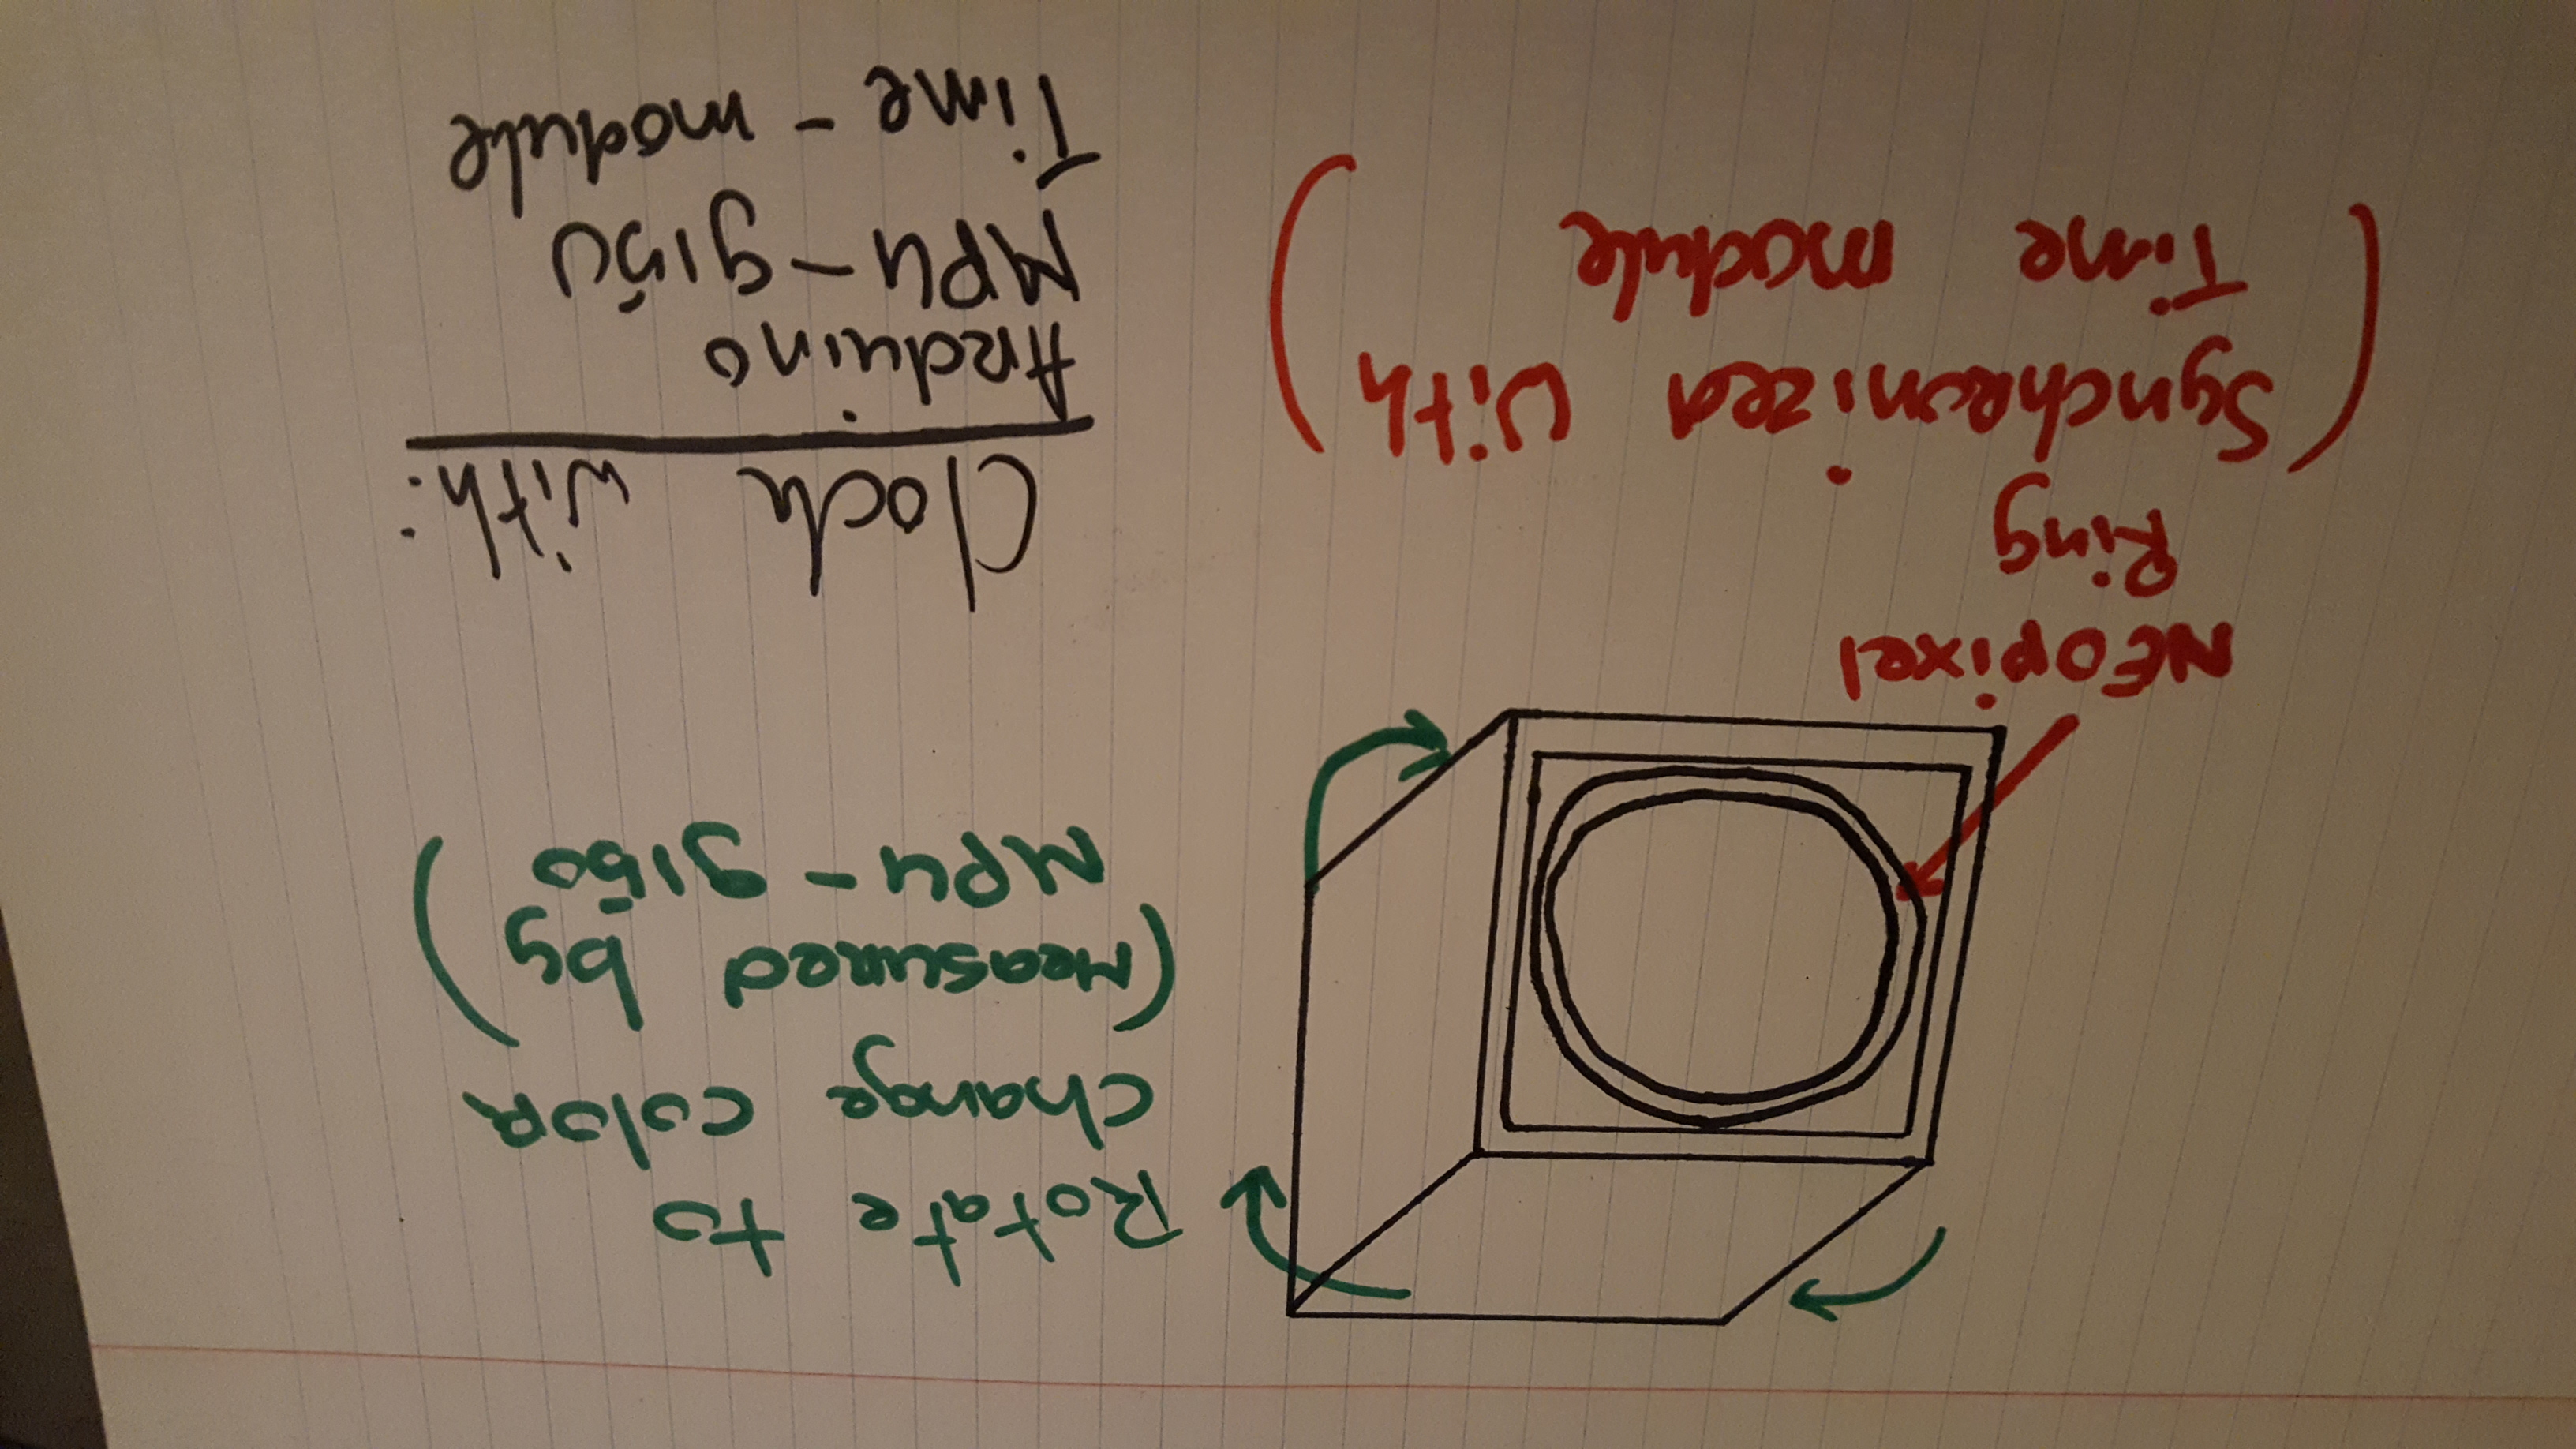
\includegraphics[scale=0.13, angle=180]{concept}
\newpage

\section{Product}
\subsection{Ontwerp}
Dit is het ontwerp van de behuizing voor de lazersnijder.
\\
\textbf{Voor de illustrator bestanden zie: \url{https://github.com/DDuunk/Clock} }
\\ \\

\includegraphics[scale=0.4]{klok}
\\ \\
Dit ontwerp heb ik uitgesneden op de lazersnijder en in elkaar gezet.
Vervolgens heb ik het goed geschuurd en ingesmeerd met meubelolie voor een betere afwerking.
Dit is het resultaat daarvan: 
\\ \\
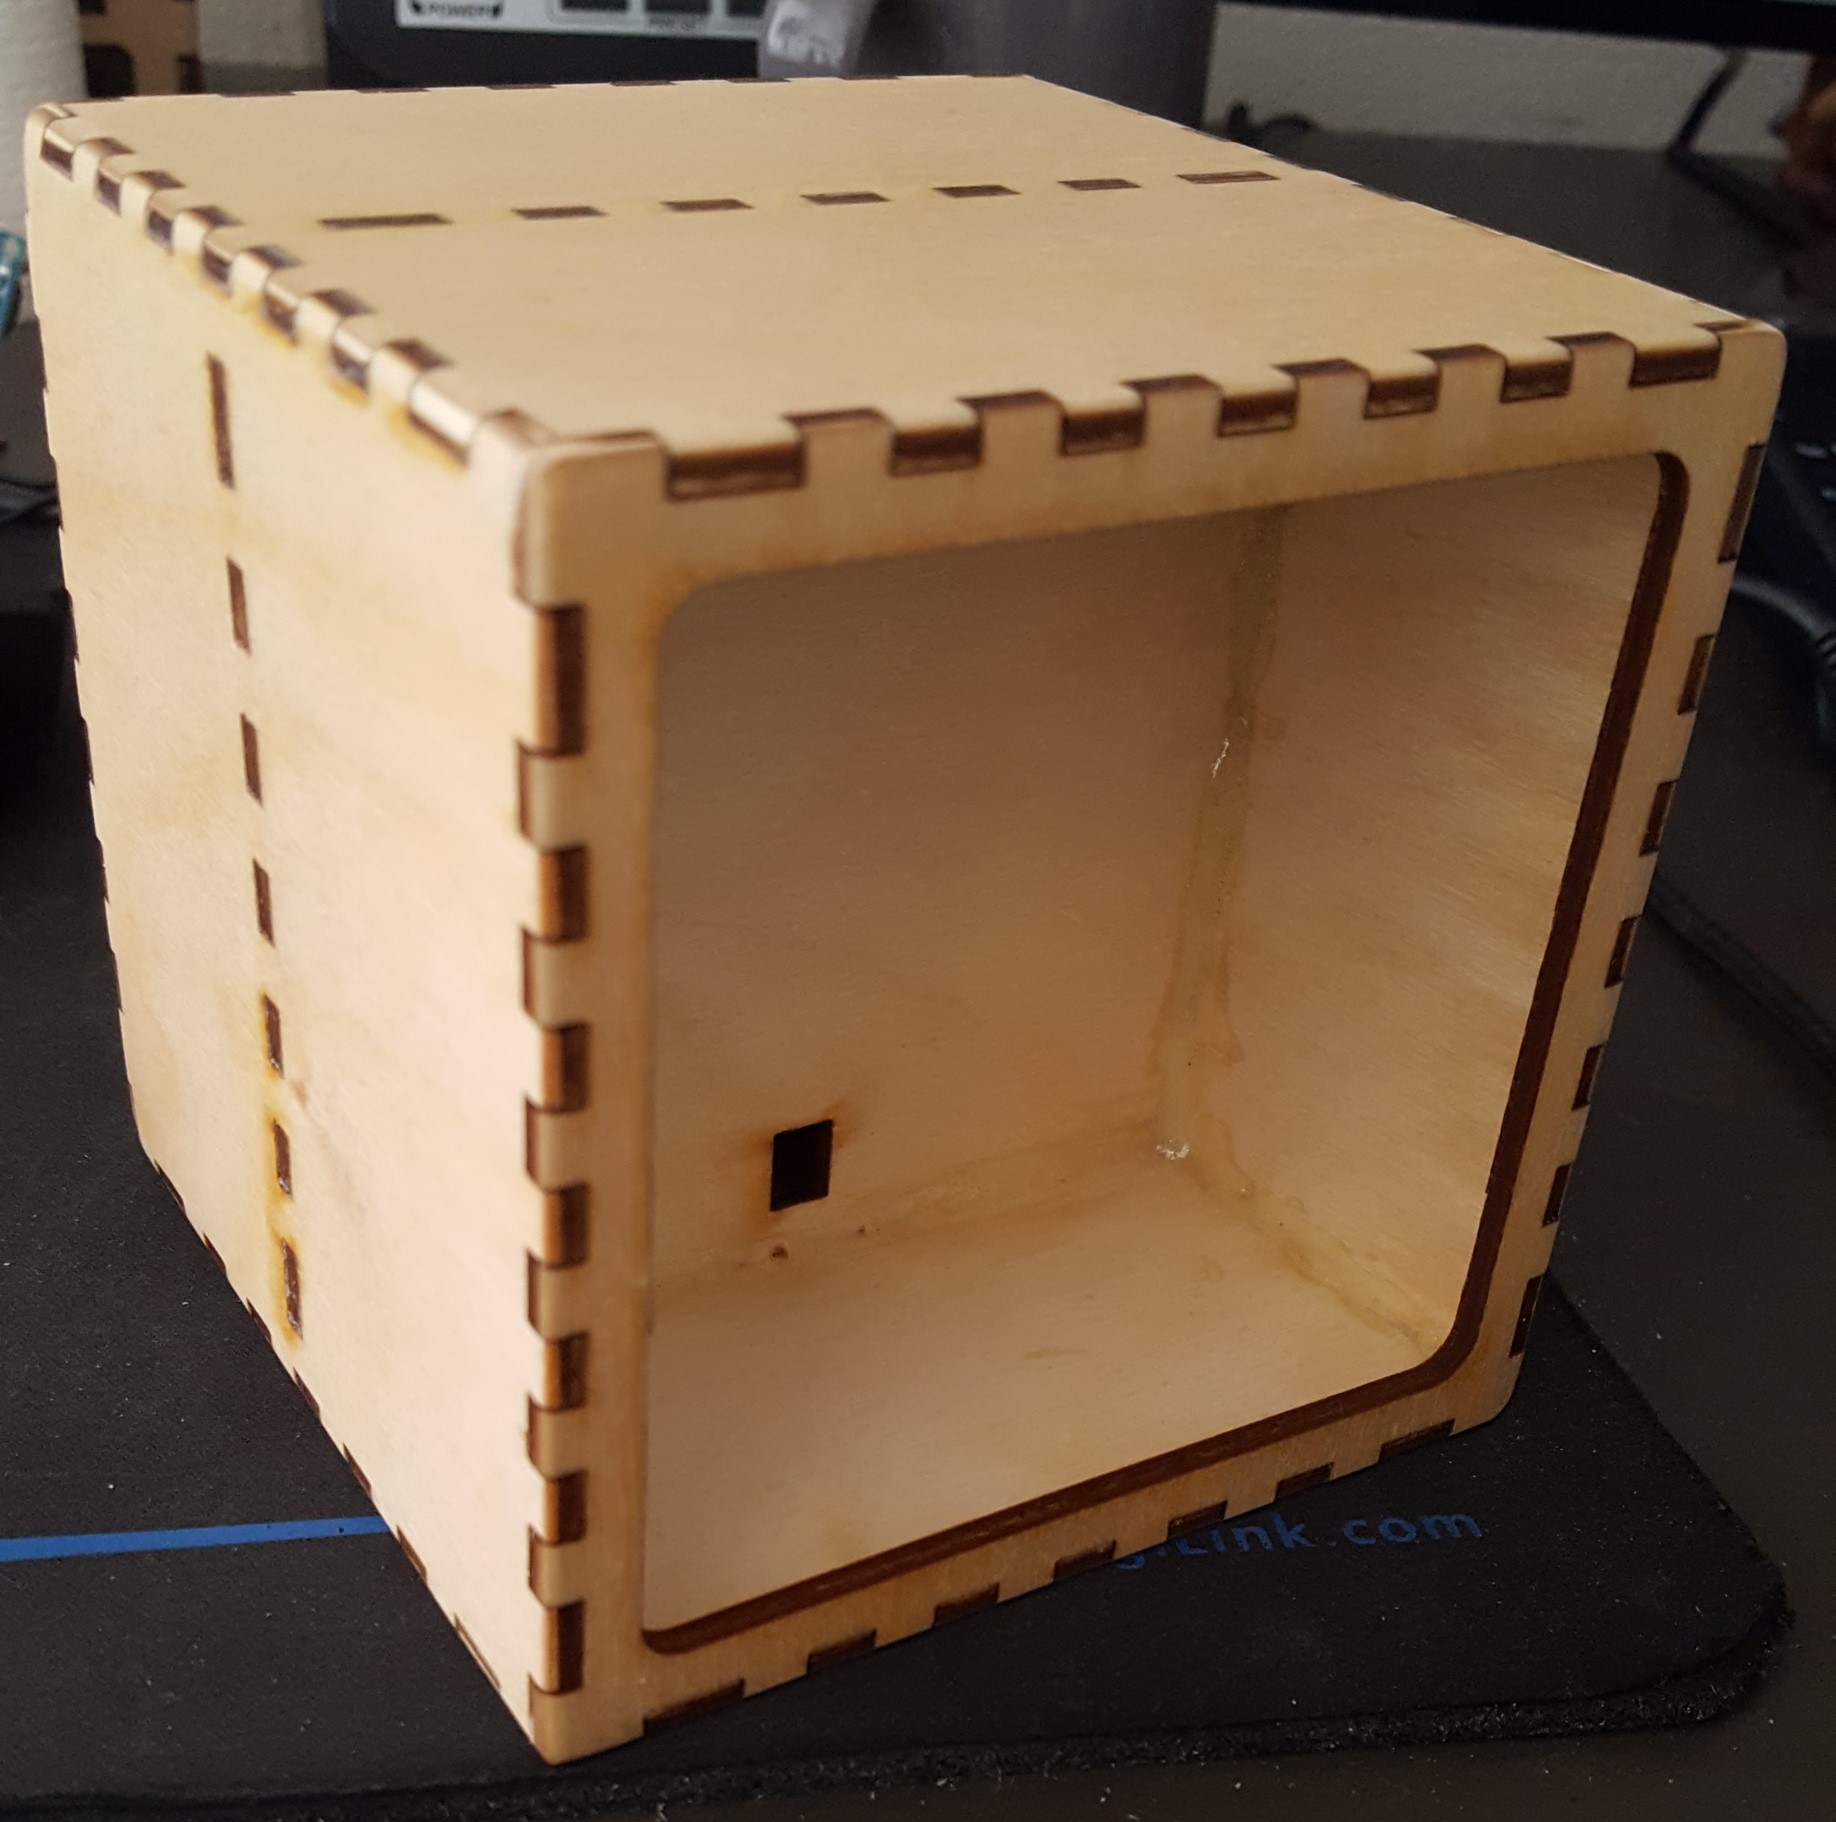
\includegraphics[scale=0.2]{case}
\subsection{Hardware}
Hier beschrijf ik de gebruikte sensoren:
\subsubsection{RTC-Module}
De RTC-Module is een tijdsensor. Deze sensor werkt ook met I2c met de Arduino. 
Het I2c adres van deze sensor is 0x68. Dit adres is van belang als er meerdere I2c apparaten worden aangesloten op de Arduino.
\newline
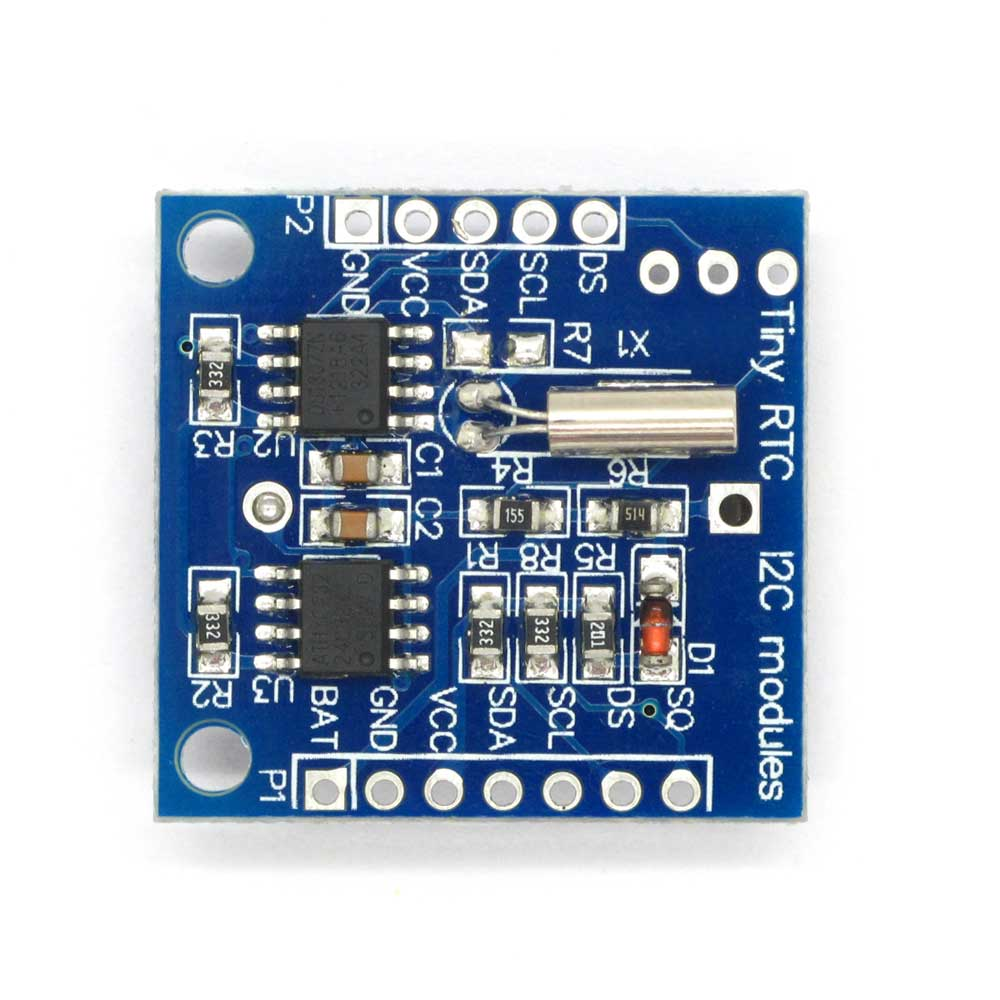
\includegraphics[scale=0.2]{RTC}
\subsubsection{MPU-9150}
De MPU-9150 is een 9-axis bewegingsregistrator sensor. Deze sensor werkt via I2c met de Arduino.
Zoals al eerder is verteld is het I2c adres van belang bij het gebruik van meerdere I2c apparaten.
Dit is waarom: De MPU-9150 gebruikt als standaard I2c adres ook 0x68 (hetzelfde adres als de RTC-Module) hierdoor onstaan problemen met sensoren uitlezen.
Gelukkig is het mogelijk om het I2c adres van de MPU-9150 te veranderen naar 0x69, dit is mogelijk door AD0 aan te sluiten op 3.3VCC. 
\newline
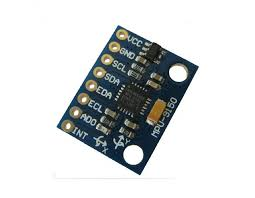
\includegraphics[scale=0.8]{MPU-9150}
\subsubsection{Elektrisch Schema}
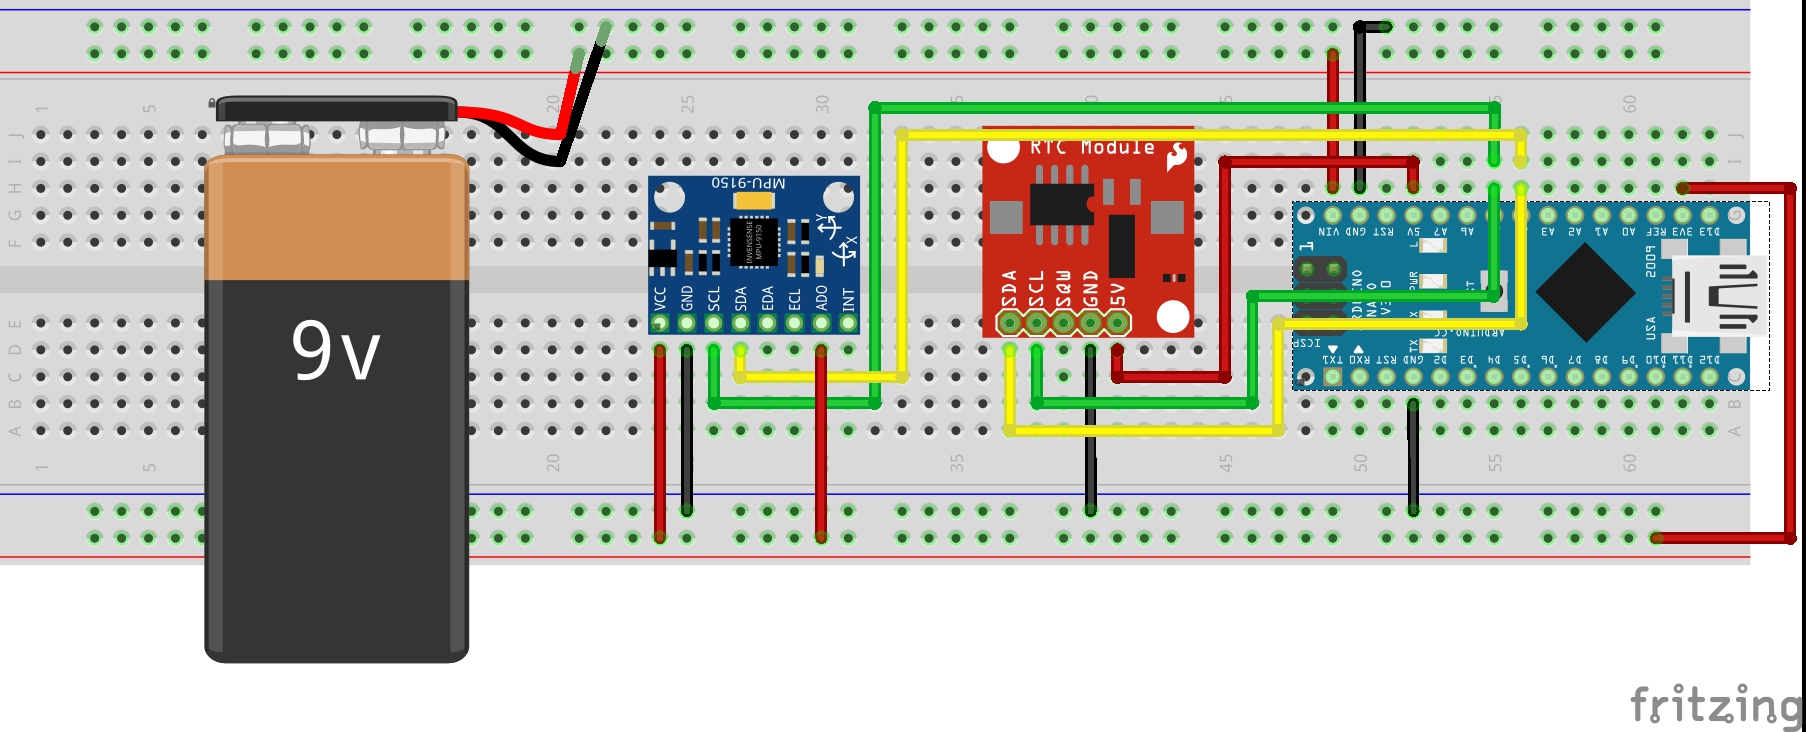
\includegraphics{circuit_bb}
\subsection{Code}
Coderen speelt een grote rol bij het ontwikkelen van een "Smart Object".
Met coderen bepaal je hoe het object werkt en hoe je het wilt gebruiken.
Hier laat ik verschillende stukken code en libraries zien.
\subsubsection{Libraries}
Voor de code heb ik gebruik gemaakt van verschillende libraries, hier zijn de belangrijkste: 
\\ \\
Library voor de NeoPixel Ring:\\
\url{https://github.com/adafruit/Adafruit_NeoPixel}
\\ \\
Libraries voor de RTC-Module:\\
\url{https://github.com/adafruit/RTClib}\\
\url{https://www.arduino.cc/en/reference/wire}
\\ \\
Libraries voor de MPU-9150:\\
\url{https://github.com/jrowberg/i2cdevlib/blob/master/Arduino/I2Cdev/I2Cdev.h}\\
\url{https://github.com/alexvonduar/mpu9150-arduino-lib/blob/master/libraries/MPU9150Lib/MPU9150Lib.h}

\subsubsection{Code fragmenten}
Dit is de code voor de afhandeling van de rotatie:
\begin{lstlisting}[caption=NEOPIXEL.cpp]
void NEOPIXEL_RUN() {
    if (MPU.xValue > 0 && MPU.xValue < 90) {
        mode = 1;
    } else if (MPU.xValue > 90 && MPU.xValue < 180) {
        mode = 2;
    } else if (MPU.xValue < 0 && MPU.xValue > -90) {
        mode = 3;
    } else if (MPU.xValue < -90 && MPU.xValue > -180) {
        mode = 4;
    }
    timeCycle(second, minute, hour, mode);
}
\end{lstlisting} 
Hier verander ik de kleur t.o.v. het variable "mode" die van het vorige stukje code afkomt.
Ook zorg ik dat de tijd over de 24 led's van de NeoPixel Ring wordt verspreidt.
\begin{lstlisting}[caption=NEOPIXEL.cpp]
void timeCycle(int sec, int min, int h, int mode) {
    switch(mode) {
        case 1: cSec = strip.Color(255, 0, 0); //red
                cMin = strip.Color(0, 255, 0); //green
                cHour = strip.Color(0, 0, 255); //blue
                break;
        case 2: cSec = strip.Color(0, 255, 0); //green
                cMin = strip.Color(0, 0, 255); //blue
                cHour = strip.Color(255, 0, 0); //red
                break;
        case 3: cSec = strip.Color(0, 0, 255); //blue
                cMin = strip.Color(255, 0, 0); //red
                cHour = strip.Color(0, 255, 0); //green
                break;
        case 4: cSec = strip.Color(255, 0, 0); 
                cMin = strip.Color(255, 255, 0); 
                cHour = strip.Color(255, 0, 255);
                break;                       
    }
      
    if(((sec - 1) / 2.5) < 0 || ((min - 1) / 2.5) < 0 ||
       ((h - 1) * 2) < 0) {
        strip.setPixelColor(23, 0, 0, 0);
        strip.show();
    } else if (((sec - 1) / 2.5) < 1 || ((min - 1) / 2.5) < 1 ||
       ((h - 1) * 2) < 1) {
        strip.setPixelColor(0, 0, 0, 0);
        strip.show();
    } else {
        strip.setPixelColor(((sec - 1) / 2.5), 0, 0, 0);
        strip.setPixelColor(((min -1) / 2.5), 0, 0, 0);
        strip.setPixelColor(((h - 1) * 2), 0, 0, 0);
        strip.show();
    }
      
    strip.setPixelColor(sec / 2.5, cSec);
    strip.setPixelColor(min / 2.5, cMin);
    strip.setPixelColor(h * 2, cHour);
    strip.show();
}
\end{lstlisting}
In dit stukje code wordt de RTC-Module gesynchronizeerd met de tijd van je computer. 
Dit gebeurt tijdens het compileren van de code.
\begin{lstlisting}[caption=RTC.cpp]
void RTC_INIT() {
    while (!Serial);
    if (!rtc.begin()) {
        Serial.println("Couldn't find RTC");
        while (1);
    }
    rtc.adjust(DateTime(F(__DATE__), F(__TIME__)));
}
\end{lstlisting}
Dit is de code om de MPU-9150 te initializeren:
\begin{lstlisting}[caption=MPU.cpp]
void MPU_INIT() {
    Serial.print("Arduino9150 starting using device "); 
    Serial.println(DEVICE_TO_USE);
    Wire.begin();
    MPU.selectDevice(DEVICE_TO_USE);
    MPU.init(MPU_UPDATE_RATE, MPU_MAG_MIX_GYRO_AND_MAG, 
             MAG_UPDATE_RATE, MPU_LPF_RATE); 
}
\end{lstlisting}
\textbf{Voor de volledige code zie: \url{https://github.com/DDuunk/Clock} }

\section{Problemen}
Tijdens het maken van het "Smart Object" ben ik op een aantal problemen beland, dit zijn deze problemen: 
\\ \\
Aangezien ik een NeoPixel Ring van 24 leds gebruik moest ik de tijd die normaal over 60 verspreid wordt omzetten naar 24.
Dit zorgte ook ervoor dat de 24ste led aan bleef staan waardoor ik in de code moest toevoegen dat als de led naar de volgende led sprong hij de vorige led uitschakelde.
Het huidige probleem is dat deze code maar tijdelijk werkt, na een tijdje blijven namelijk alle leds aan staan. Dit heeft te maken met een fout in het algoritme.

\section{Resultaat}
Dit is het resultaat van mijn "Smart Object": 
\\ \\
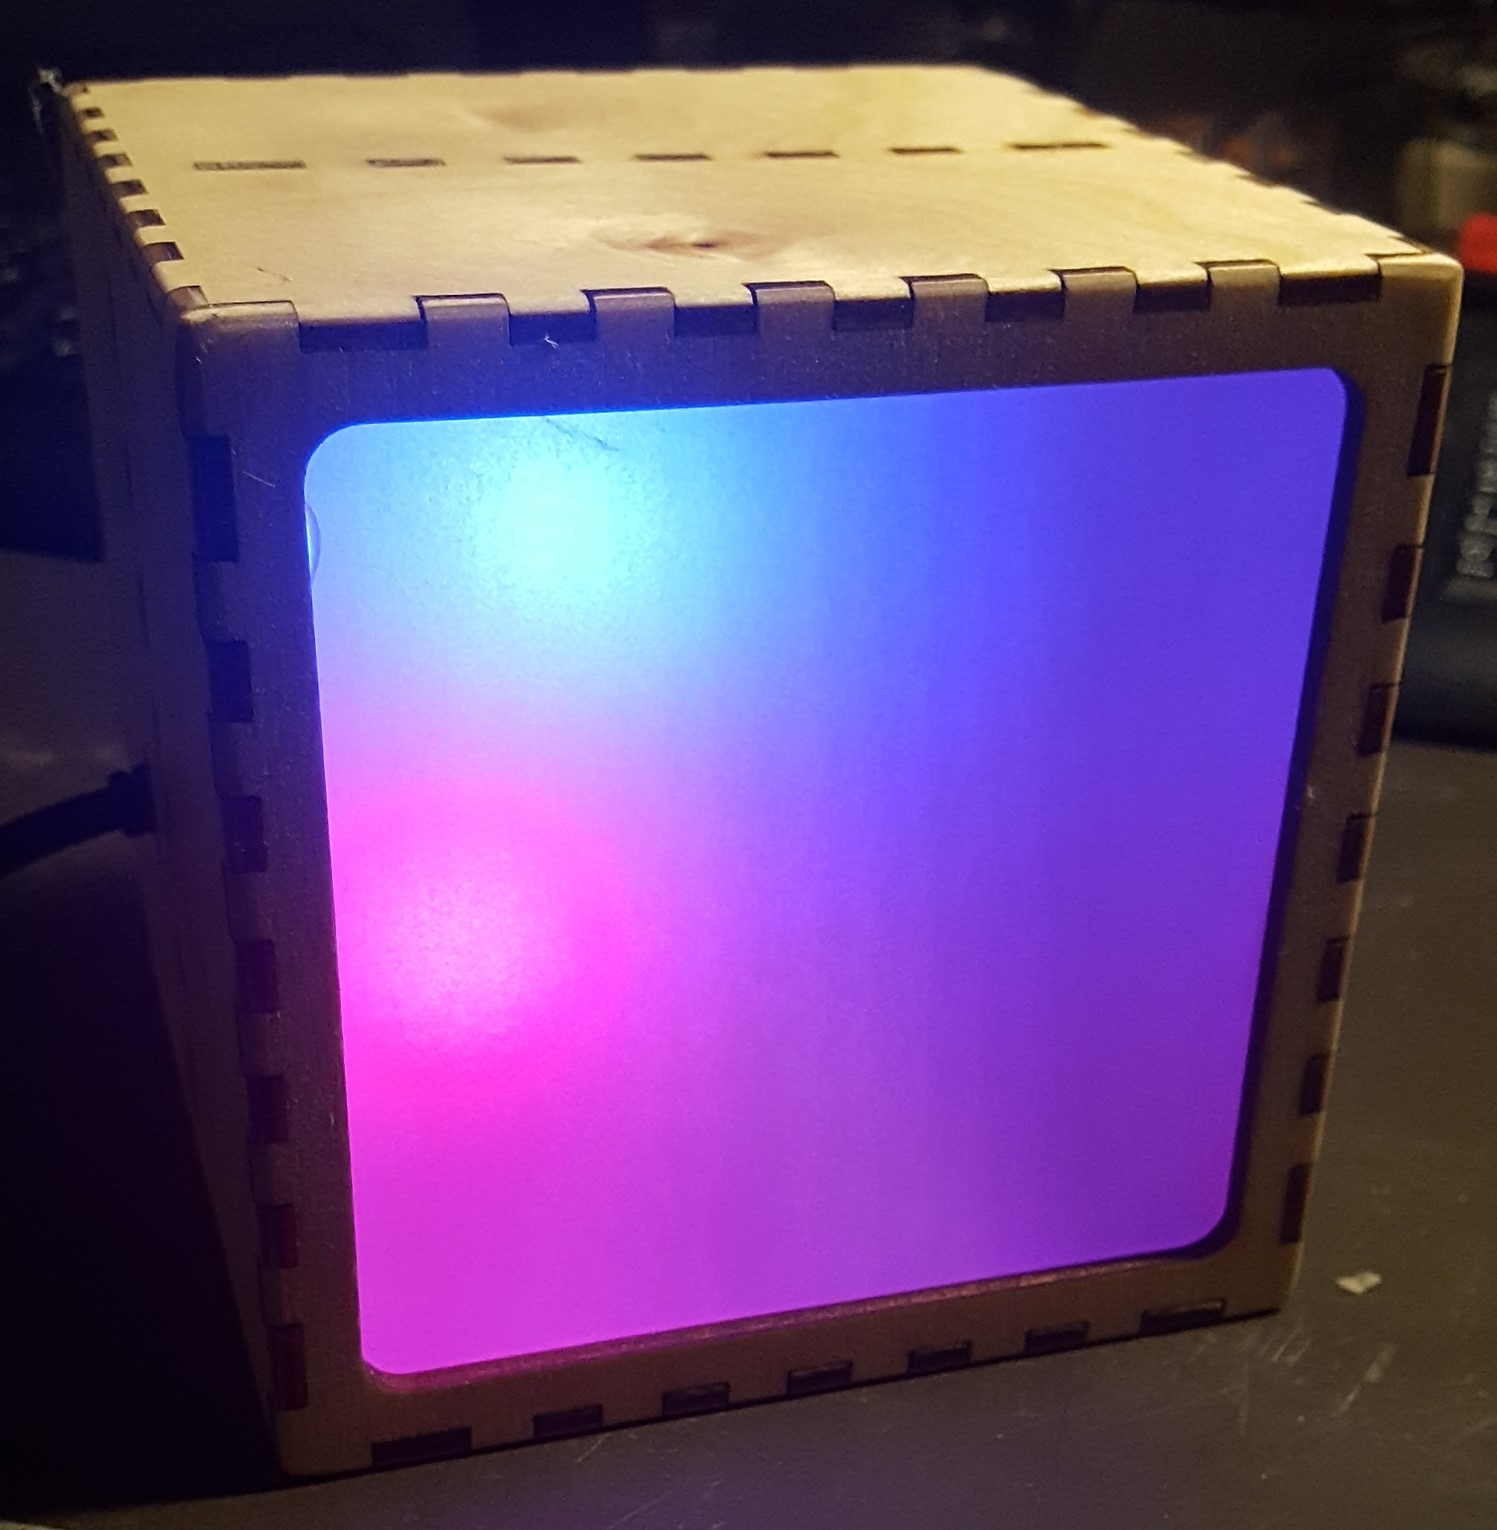
\includegraphics[scale=0.15]{resultaat1}
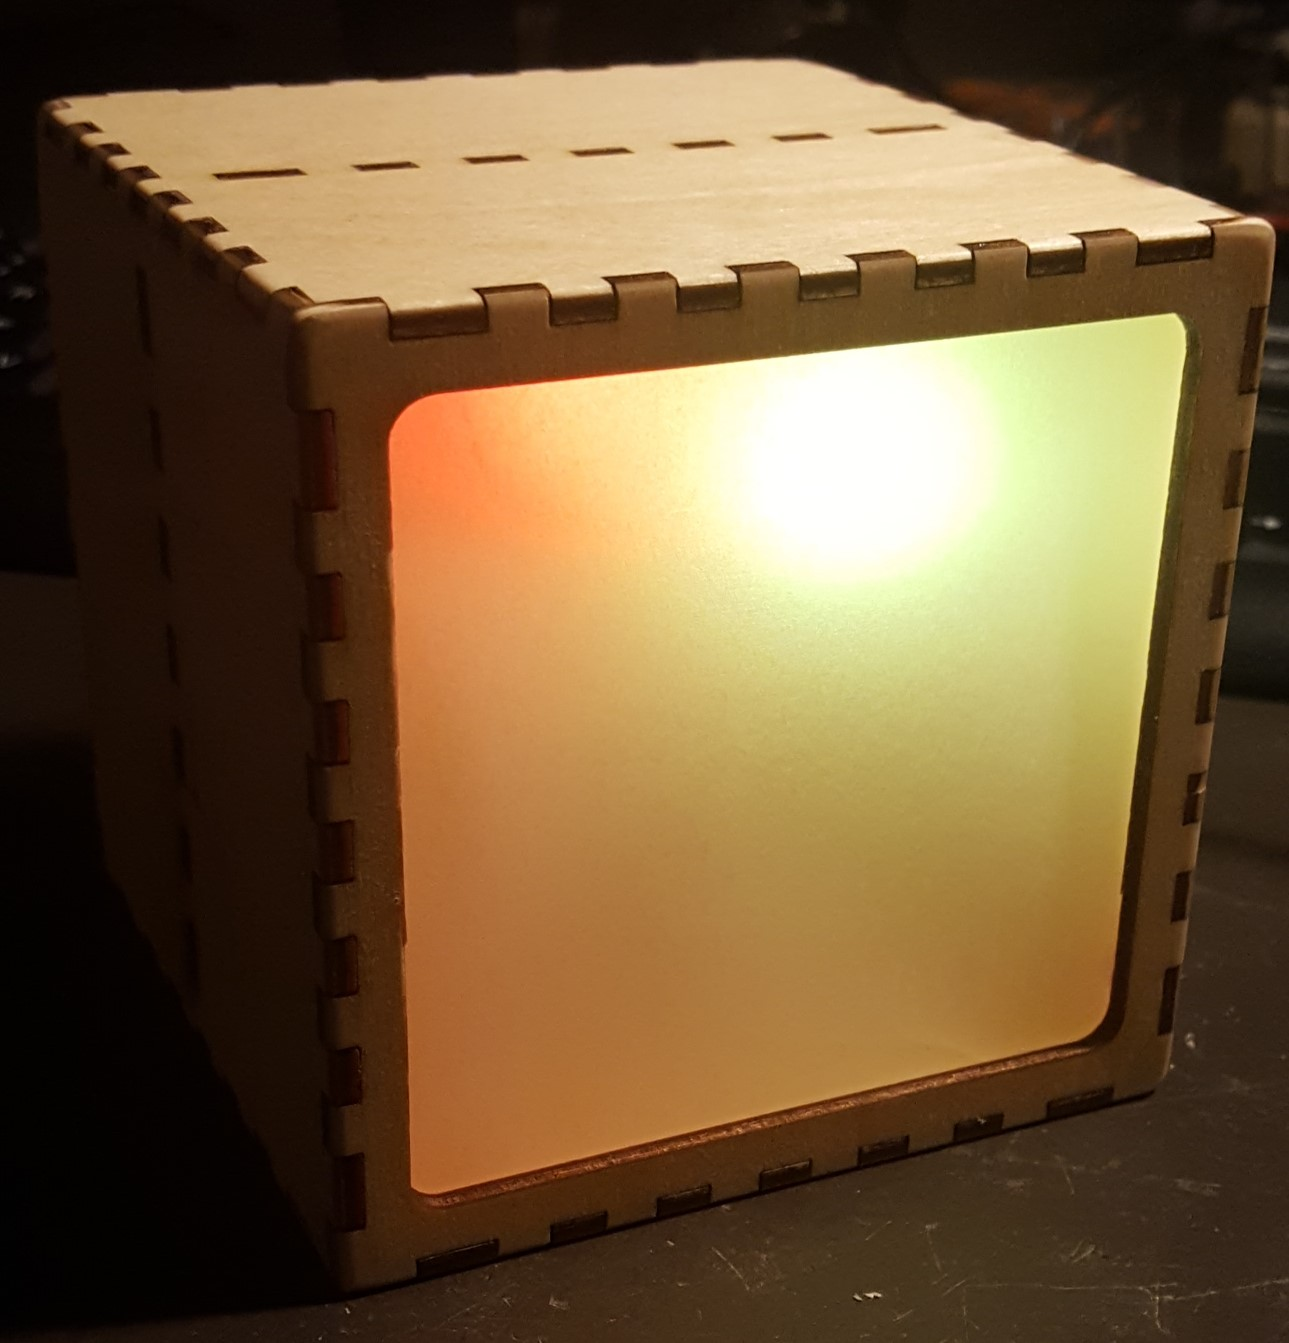
\includegraphics[scale=0.171]{resultaat2}
\end{document}